\documentclass{article}
\usepackage{graphicx}
\usepackage[T1,T2A]{fontenc}
\usepackage[utf8]{inputenc}
\usepackage[russian]{babel}
\usepackage{amsmath}
\usepackage{mathtools}
\usepackage[unicode, pdftex]{hyperref}

\title{B Plus Tree}

\begin{document}

\maketitle

\section{Вступление}
\subsection{Определение}
Для того чтобы разобраться с концепцией B+-дерева, сначала стоит подробнее изучить понятие стандартного B-дерева.

B-дерево представляет собой строго сбалансированную древовидную структуру данных, которая поддерживает отсортированные данные и разрешает поиск, последовательный доступ, вставку и удаление в логарифмическом времени. B-дерево обобщает двоичное дерево поиска, позволяя использовать узлы с более чем двумя дочерними элементами.  

Дерево является B-деревом порядка m, если обладает следующими свойствами:
\begin{itemize}
\item B-дерево является идеально сбалансированным, то есть глубина всех его листьев одинакова. 
\item Все узлы, кроме корня должны иметь как минимум [m/2] – 1 ключей и максимум m-1 ключей. 
\item Все узлы без листьев, кроме корня (т.е. все внутренние узлы), должны иметь минимум [m/2] потомков. 
\item Если корень – это узел не содержащий листьев, он должен иметь минимум 2 потомка. 
\item Узел без листьев с m-1 ключами должен иметь m потомков. 
\item Левое поддерево узла будет иметь меньшие значения, чем правая сторона поддерева. Это означает, что узлы также сортируются в порядке возрастания слева направо.
\end{itemize}

\begin{figure}
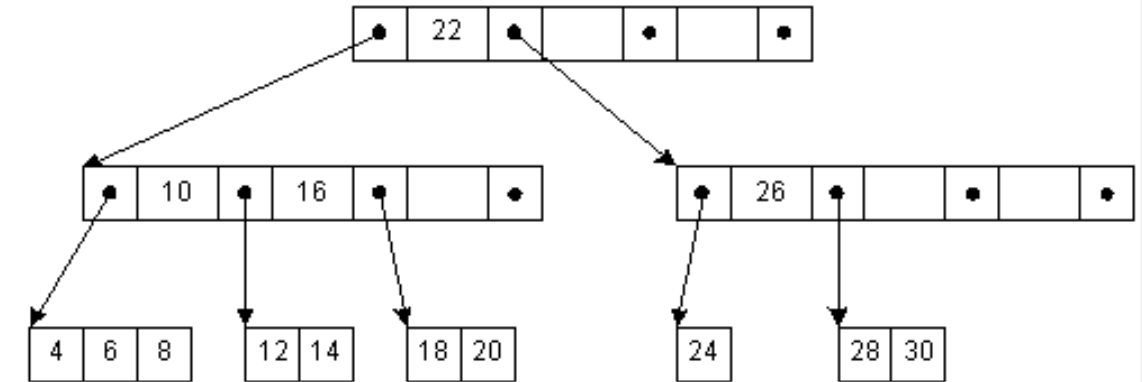
\includegraphics[scale=0.5]{1.png}
\caption{\textit{Дерево В порядка m=4}}
\end{figure}

B + -дерево является модификацией B-дерева. В B+-дереве настоящие ключи хранятся лишь в листьях дерева, а во внутренних узлах хранятся лишь ключи-маршрутизаторы, необходимые для поиска по дереву. 

Кроме свойств, наследуемых от B-дерева, B+-дерево также имеют следующие характеристики, позволяющие эффективно выполнять операции над ним:
\begin{itemize}
\item В дереве B+ записи (указатели на данные) могут храниться только на листовых узлах, а внутренние узлы могут хранить только копии ключей (значения без указателя на данные).  Здесь можно отметить, что, поскольку указатели данных присутствуют только в листовых узлах, конечные узлы обязательно должны хранить все значения ключей вместе с соответствующими указателями данных на блок дискового файла, чтобы получить к ним доступ. 
\item Листовые узлы дерева B+ связаны друг с другом в виде односвязных списков, чтобы сделать поисковые запросы более эффективными. 
\end{itemize}

\begin{figure}
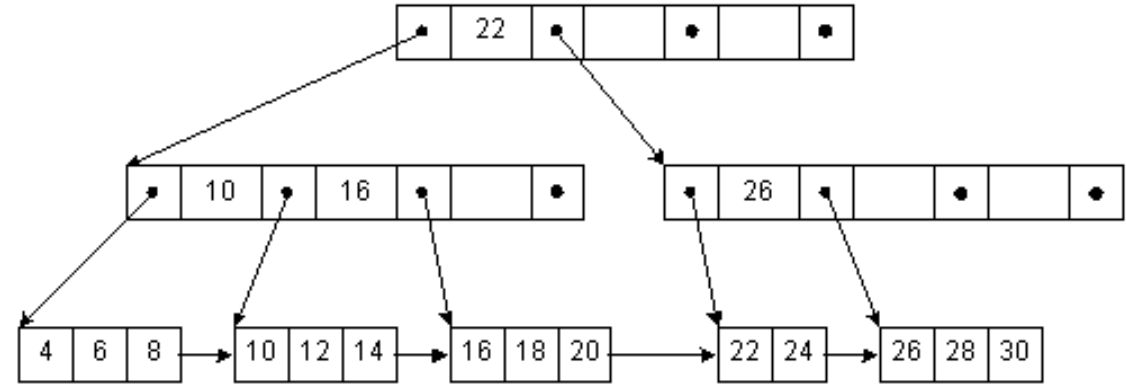
\includegraphics[scale=0.5]{2.png}
\caption{\textit{Дерево В+ порядка m=4}}
\end{figure}

\subsection{История}
B-деревья были изобретены Рудольфом Байером и Эдвард МакКрейт во время работы в Boeing Research Labs, для цели эффективного управления страницей индексов для больших файлов с произвольным доступом. Основное предположение заключено в том, что индексы могут быть настолько объемными, что в основную память поместиться лишь небольшие фрагменты дерева. Статья Байера и МакКрайта «Организация и поддержка упорядоченных индексов» была впервые распространена в июле 1970 года и позже опубликована в Acta Informatica.

Байер и МакКрайт никогда не объясняли, что означает буква B: Boeing, сбалансированный, широкие, пушистые и байеровские. МакКрайт сказал, что «чем больше вы думаете о том, что означает B в B-деревьях, тем лучше вы понимаете B-деревья».

Одной из первых статей, в которой были подробно разобраны концепции модификаций B-дерева (в том числе и B+-дерева), является статья Дугласа Комера "Вездесущее B-дерево". В этой же работе он отмечает, что B+-дерево использовалось в программном обеспечении IBM для доступа к данным VSAM, и ссылается на опубликованную в журнале IBM System Journal статью 1973 года "Рекомендации по дизайну индексации".

\subsection{Применение}
Изначально структура B+-деревьев предназначалась для хранения данных в целях эффективного поиска в блочно-ориентированной среде хранения — в частности, для файловых систем; применение связано с тем, что в отличие от бинарных деревьев поиска, B+-деревья имеют очень высокий коэффициент ветвления (число указателей из родительского узла на дочерние, обычно порядка 100 или более), что снижает количество операций ввода-вывода, требующих поиска элемента в дереве.

Структура широко применяется в файловых системах — NTFS, ReiserFS, NSS, XFS, JFS, ReFS используют этот тип дерева для индексирования метаданных; BeFS также использует B+-деревья для хранения каталогов. Реляционные системы управления базами данных, такие как DB2, Informix, Microsoft SQL Server, Oracle Database (начиная с версии 8), Adaptive Server Enterprise и SQLite поддерживают этот тип деревьев для табличных индексов. Среди NoSQL-СУБД, работающих с моделью «ключ — значение», структура данных реализована для доступа к данным в CouchDB и Tokyo Cabinet.

\section{Описание алгоритма}
\subsection{Ассимптотическая сложность}
B+-деревья являются сбалансированными, поэтому время выполнения стандартных операций в них пропорционально высоте, то есть O(logn). Однако стоит заметить, что так как степень дерева зачастую выбирается большой, константа при выполнении операций тоже большая. Это связано с большим количеством ключей в узлах, которые необходимо сравнить. Но из-за небольшой высоты дерева это не сильно сказывается на скорости работы

\subsection{Поиск}
\textit{Поиск листа}. Для того, чтобы найты нужный ключ, необходимо сначала добраться до листового узла, который может его содержать. С помощью бинарного или линейного поиска ищется интервал содержащий значение ключа и осуществляется переход к соответствующему сыну. Операция повторяется пока текущий узел не окажется конечным(листовым). Функция возвращает лист, содержащий ключ. В противном случае пользователю показывается неудачная попытка.

\textit{Поиск ключа}. Производится поиск листа и последующий поиск искомого ключа в нем. Программа выдает индекс искомого ключа и показывает неудачную попытку в противном случае.

Далее будет разобран пример поиска ключа k=4 в B+-дереве порядка m=3.

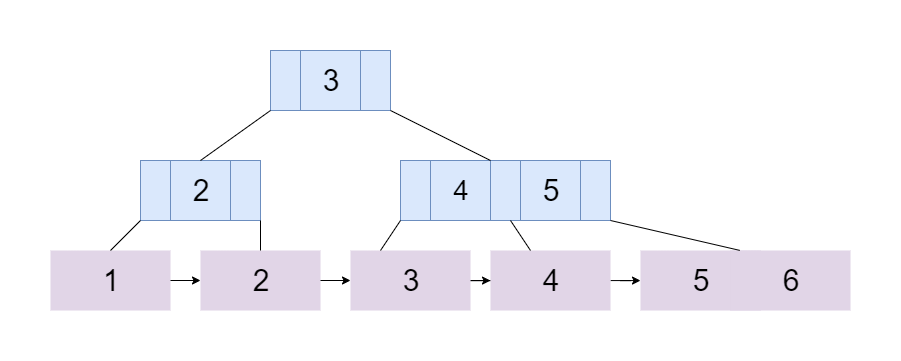
\includegraphics[scale=0.4]{bsearch.png}

Необходимо сравнить k=4 с корневым узлом. Так как k>3, осуществляется переход к правому потомку.

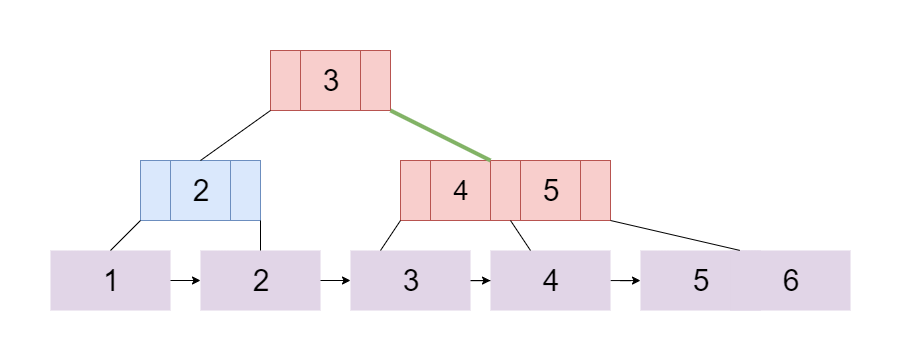
\includegraphics[scale=0.4]{bsearch2.png}

Необходимо найти нужный интервал. Так как k>=4, значение ключа сравнивается с следующим элементом: k<=5. Значит, осуществляется переход в подинтервал $[4; 5]$ и производится поиск единственного ключа, соответствующего искомому. Операция завершена.

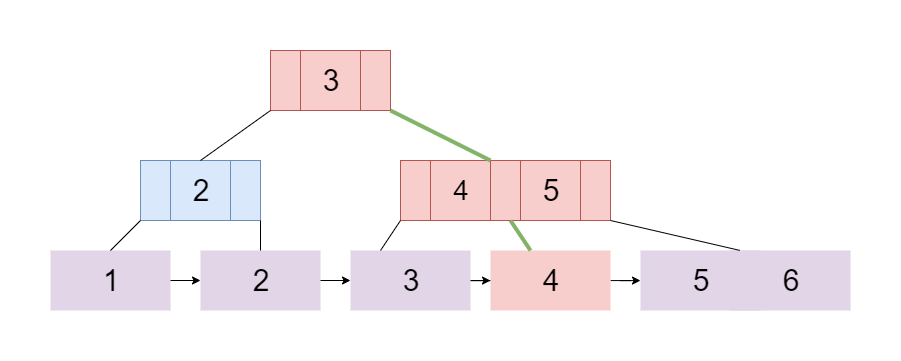
\includegraphics[scale=0.4]{bsearch3.png}

\subsection{Добавление}
Если дерево пустое, нужно создать новый корень и добавить первый ключ.

 Иначе производится поиск листа, в который можно добавить ключ. Ключ добавляется в список в порядке неубывания. Если лист не заполнен, операция завершена. В случае, если лист заполнен, последующим действием после вставки выполняется \textit{разбиение узла}.

Узел делится на две половины. Элемент m/2+1 переносится в родительский узел. Если родительский узел оказывается заполненным, повторяется \textit{разбиение узла}.

Далее на примере дерева порядка m=3 будут рассмотрены два случая: когда количество элементов узла меньше m+1 и когда происходит переполнение узлов.


\textit{1 случай.} Производится поиск нужного листа и добавление k=2 в порядке возрастания.

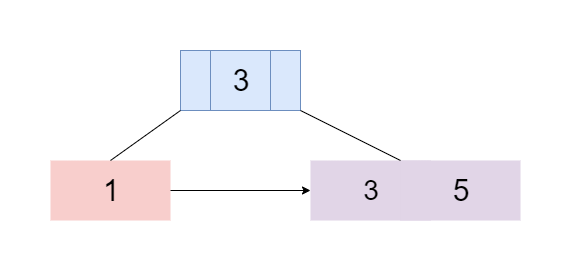
\includegraphics[scale=0.4]{binsert11.png}

При добавлении количество элементов не превышает максимальное. Значит, операция завершается.

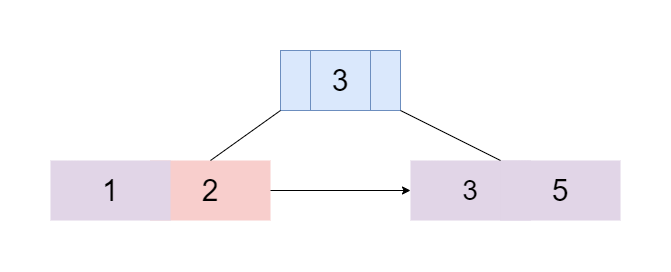
\includegraphics[scale=0.4]{binsert2.png}

\textit{2 случай.} Производится поиск нужного листа и добавление k=6 в порядке возрастания.

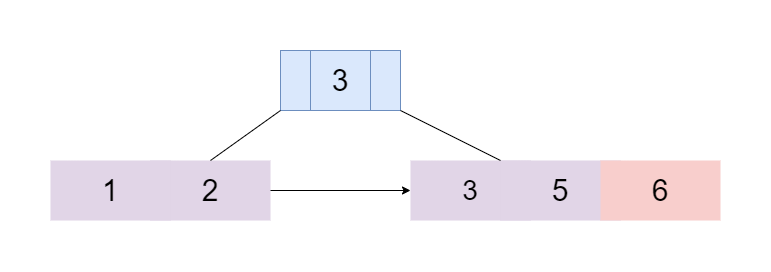
\includegraphics[scale=0.4]{binsert21.png}

Сейчас в текущем листе содержится слишком много ключей, поэтому необходимо разбить его на два. Берется ключ под номером $[k/2+1]$ со значением 5 и его копия помещается в родительский узел.

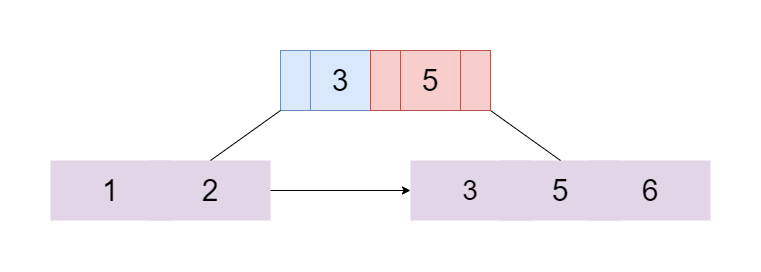
\includegraphics[scale=0.4]{binsert22 (1).png}

В левый узел помещается $[n/2]$, а в правый $[n/2+1]$ ключей (где n - изначальное количество ключей).

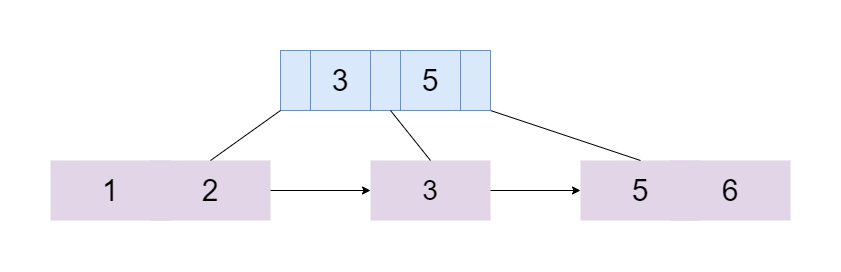
\includegraphics[scale=0.4]{binsert23 (1).png}

В родительском узле количество ключей не превышает норму, поэтому операция завершается.

\subsection{Удаление}
  Поскольку все ключи находятся в листах, для удаления в первую очередь необходимо найти листовой узел, в котором он находится, а затем и сам ключ. При нахождении нужного ключа он и связанная с ним ссылка удаляются. Если узел содержит минимальное количество ключей операция завершается. В противном случае нужно провести балансировку дерева.

  Для этого производится попытка перераспределения элементов, то есть добавления в узел элемент из левого или правого брата (не забыв обновить информацию в родителе). Если это невозможно, необходимо выполнить слияние с братом и удалить ключ, который указывает на удалённый узел. Объединение может распространяться на корень, тогда происходит уменьшение высоты дерева.

   Далее будут разобраны три случая.

   \textit{1 случай.} Ключ, который нужно удалить, присутствует только в листовом узле, а не во внутренних узлах. Для этого есть два случая:
   
   1.Удаляется ключ со значением k=7. 

   \includegraphics[scale=0.4]{dell1.png}

   Так количество ключей в узле соответствует минимальному, операция завершается.
   
   \includegraphics[scale=0.4]{dell2.png}

   2.Удаляется ключ k=5. При удалении в узле количество ключей становится меньше минимального.
   
      \includegraphics[scale=0.4]{dell3.png}
      
      \includegraphics[scale=0.4]{dell4.png}

  Добавляется срединный ключ потомка к родителю.

      \includegraphics[scale=0.4]{dell5.png}

    Недостающий заимствуется ключ у брата. 

       \includegraphics[scale=0.4]{dell6.png}

   
   

   \textit{2 случай.}Ключ, который нужно удалить, присутствует и во внутренних узлах. Имеются следующие случаи для этой ситуации.
   
   1.Удаляется ключ k=7.

   \includegraphics[scale=0.4]{dell11.png}
   
   Если количество ключей в узле больше минимального, ключ просто удаляется из листового и внутреннего узла.

   \includegraphics[scale=0.4]{dell22.png}
   
Пустое место во внутреннем узле заполняется преемником по порядку.

\includegraphics[scale=0.4]{dell33.png}

2.Удаляется ключ k=3.

\includegraphics[scale=0.4]{dell111.png}

Ключ удаляется и новый заимствуется у его родственного узла, если в нем после этого будет минимальное количество ключей.

\includegraphics[scale=0.4]{dell222.png}

Пустые узлы заполняются заимствованным ключом.

\includegraphics[scale=0.4]{dell333.png}

\textit{3 случай.} Удаляется ключ k=8, который содержится в листовом и внутреннем узле. Позаимствовать ключи у соседних братьев невозможно, так как тогда их количество ключей будет меньше минимального. 

\includegraphics[scale=0.4]{ddel1.png}

Создается пустое пространство, ссылки на которое в последующем удаляются.

\includegraphics[scale=0.4]{ddel2.png}

Далее проделывается слияние корня и ближайшего незаполненного ребенка.

\includegraphics[scale=0.4]{ddel3.png}

Создаются новые ссылки, старые удаляются.

\includegraphics[scale=0.4]{ddel4.png}


 
\section{Постановка задачи}
\textbf{Условие задачи} 

Необходимо реализовать m-арное дерево поиска, удовлетворяющее следующим условия:
\begin{itemize}
\item Дерево строго сбалансировано (каждая ветвь имеет одну высоту)
\item Каждый узел имеет m дочерних элементов и m-1 ключей или их копий
\item Во внутренних узлах хранятся только копии ключей, сами ключи лежат в листьях. Листовые узлы представляют собой односвязный список
\end{itemize}

А также выполняемое следующие операции над собой:
\begin{itemize}
    \item insert(int k) - добавляет ключ k в дерево
    \item delete(int k) - удаляет ключ k из дерева
    \item findkey(int k) - ищет ключ по значению и в случае успеха возвращет True, иначе - False
    \item print() - обходит каждый узел начиная с левого поддерева и выводит построчно списки ключей или их копий.
\end{itemize}

\textbf{Формат входных данных:}

В первой строке входные данные имеют число m (степень дерева). Далее пользователем в консоль вводятся команды в формате строки. Вызов операций вставки, удаления и поиска имеет вид \textbf{\{"название команды" \quad k\}}, где k - ключ. Чтобы программа завершилась, необходимо ввести в консоль "end".

\textbf{Формат выходных данных:}

После того как пользователь вызовет команду завершения, в консоли отобразятся ключи каждого узла, начиная с левого поддерева.

\textbf{Ограничения:}

2 $\leq$ m $\leq$ 100

$-2^{31}$ < k < $2^{31}$
\section{Заключение}

Таким образом, B+-деревья являются актуальной структурой данных, с помощью которой можно эффективно и последовательно обрабатывать большие объемы данных с сохранением логарифмической сложности.

\section{Список литературы}
\begin{enumerate}
\item B.Bayer, E.McCreight "Organization and maintenance of large ordered indices"
\item WAGNER, R. "Indexing design considerations," IBM Syst. J. 4, (1973)
\item "The Ubiquitous B-Tree " DOUGLAS COMER Computer Sctence Department, Purdue Untverstty, 
\item Т. Кормен, Ч. Лейзерсон, Р. Ривест, К. Штайн. Алгоритмы: построение и анализ. 3-е изд. 
\item DOUGLAS COMER: "The Ubiquitous B-Tree", Computer Sctence Department, Purdue Untversty
\item Дональд Кнут. Генерация всех деревьев. История комбинаторной генерации 
\item Зубов В. С., Шевченко И. В. "Структуры и методы обработки данных: Практикум в среде Delphi" Глава 6. Поиск в недвоичных деревьях - B-деревьях 
\item Freitas R, Wilcke W. Storage-class memory: The next storage system technology. IBM Journal of Research and Development, 2008 
\item \url{https://ru.wikipedia.org/wiki/B-%D0%B4%D0%B5%D1%80%D0%B5%D0%B2%D0%BE}
\item \url{http://algolist.manual.ru/ds/s_btr.php}
\item \url{https://www.bluerwhite.org/btree/}
\item \url{https://neerc.ifmo.ru/wiki/index.php?title=B%2B-%D0%B4%D0%B5%D1%80%D0%B5%D0%B2%D0%BE}
\item \url{Kerttu Pollari-Malmi "B+-trees"}
\item \url{https://www.youtube.com/watch?v=DqcZLulVJ0M}
\item \url{https://www.youtube.com/watch?v=pGOdeCpuwpI}
\item \url{https://www.youtube.com/playlist?list=PLsEFMZUL5KsOqKHhxquVleVkM9LFLFSo0}
\item \url{https://cs.hse.ru/data/2019/04/08/1176295299/%D0%A0%D0%B8%D0%B3%D0%B8%D0%BD_CoCoS_2019.pdf}
\item \url{https://www.scaler.com/topics/data-structures/b-plus-trees/}
\item \url{https://stackoverflow.com/questions/870218/what-are-the-differences-between-b-trees-and-b-trees}
\item \url{http://algolist.manual.ru/ds/s_btr.php}
\item \url{https://thodrek.github.io/cs564-fall17/lectures/lecture-14/Lecture_14_Hash.pdf}
\item \url{https://www.usenix.org/publications/loginonline/revisit-b-tree-vs-lsm-tree-upon-arrival-modern-storage-hardware-built}
\item \url{https://www.w3schools.blog/b-plus-tree-dbms}
\item \url{https://www.youtube.com/watch?v=TdtulzNC9iE}
\item \url{https://www.youtube.com/watch?v=KFcpDTpoixo&t=1s}
\item \url{https://www.programiz.com/dsa/insertion-on-a-b-plus-tree}
\item \url{https://www.cs.usfca.edu/~galles/visualization/BPlusTree.html}

\end{enumerate}

\end{document}


